\chapter{插图插表及引用方法(仅供参考)}


\section{插图}
插图:一般情况下,在正文中,先见到图号和图的内容再展示图。
特殊情况须延后的插图不应跨节。

通常使用的函数图采用简化形式,称为简写函数图,例如图{\ref{fig:historyhebut}}。
\begin{figure}[ht]
    \centering
    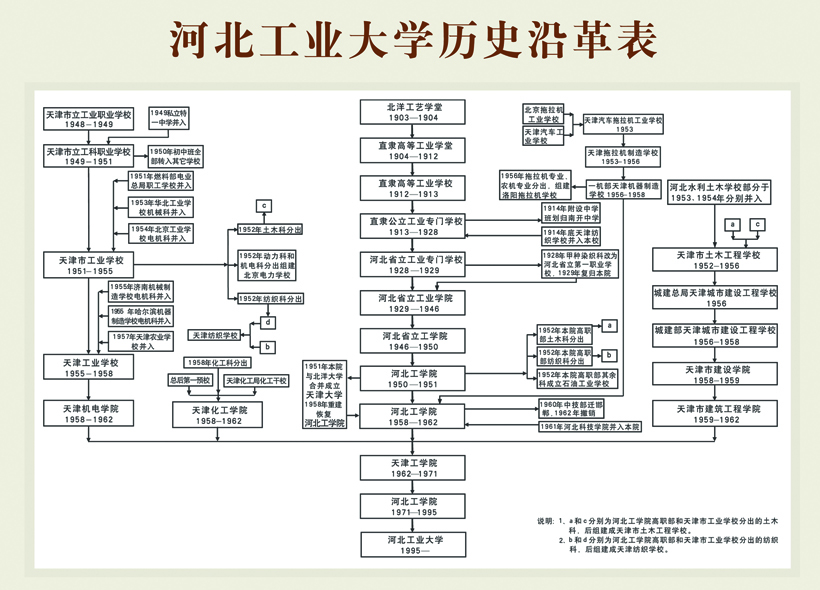
\includegraphics[width=0.5\textwidth]{figures/historyhebut}
    \caption{河北工业大学历史沿革}\label{fig:historyhebut}
\end{figure}


\section{插表}
一般情况下,表格须通栏,即表格宽度与正文版面平齐,如下表所示。
\begin{table}
    \centering
    \caption{测试用例表}\label{tab:table_centered}
    \begin{tabularx}{\textwidth}{>{\centering\arraybackslash}X>{\centering\arraybackslash}X>{\centering\arraybackslash}X}
    \toprule
    列1 & 列2 & 列3 \\
    \midrule
    有效 & 001 & 通过 \\
    无效 & 002 & 未通过 \\
    \bottomrule
    \end{tabularx}
\end{table}

\section{引用}
引用如这样\cite{song_score-based_2020}